\chapter{Unidad 4}
% Falta por hacer
% Subestaciones de distribución MT/MT. Juego de barras.  Materiales y construcciones normales. Protección contra sobrecorriente transformadores y distribuidores. Protección contra sobretensiones: Selección de descargadores. Riesgo del uso de la energía eléctrica. Tensión de paso, de contacto y transferida. Sistema de puesta a tierra
% Hecho:
% Centros de transformación MT/BT. Celdas primarias y secundarias en MT (no la distinción entre primaria y secundaria).

\section{Centros de transformación}

Según la AEA-95401 (\cite{aea95401}) un \acrfull{ct} es una ``instalación destinada a transformar la energía eléctrica de una valor de tensión de \acrshort{mt} a otro valor de
tensión de \acrshort{mt} o \acrshort{bt}. o viceversa. Incluye el/los transformador/es,el equipamiento de maniobra y protección, y la estructura que contiene o soporta el equipamiento''. También se denomina como subestación de distribución.


Entonces, los elementos básicos de un CT son:

\begin{itemize}
	\item Equipos de \acrshort{mt}.
	\item El o los transformadores.
	\item Equipos de \acrshort{bt}.
\end{itemize}

\subsection{Clasificación de los CT}

Se clasifican, de acuerdo con la tabla \ref{tab:clas-ct}, dependiendo de su misión y su situación en la red eléctrica de \acrshort{at}.

\begin{longtable}{ll}
	\caption{Clasificación de los CT}\label{tab:clas-ct}\\
	\hline
	\endfirsthead
	\multicolumn{2}{l}{\cabezaTabla{tab:clas-ct}}\\\hline
	\endhead
	\hline
	\multicolumn{2}{r}{\pieTabla}
	\endfoot
	\hline
	\endlastfoot
	\multirow{3}{*}{Por alimentación} & CT alimentado en punta \\
	& CT alimentado en paso, en anillo o en bucle\\
	& CT de maniobra (o reparto)\\\hline
	\multirow{2}{*}{Por la propiedad} & CT de compañía \\
	& CT de cliente o abonado \\\hline
	\multirow{2}{*}{Por el emplazamiento} & CT de intemperie \\
	& CT de interior \\\hline
	\multirow{2}{*}{Por el tipo de acometida} & CT con acometida aérea \\\noalign{\penalty10000} % Para que no corte en la mitad del multirow
	& CT con acometida subterránea \\\hline
	\multirow{3}{*}{Por la obra civil} & CT convencional \\
	& CT prefabricado \\
	& CT subterráneo
\end{longtable}

\subsubsection{Por alimentación}

\begin{itemize}
	\item Un CT alimentado \textbf{en punta} está ubicado al final de una línea, o bien es único en dicha línea. En este último caso se suele denominar independiente. Sólo tiene una entrada de línea.
	
	\item Un CT \textbf{de paso} están ubicados en un punto medio de una línea. A ellos llega una línea desde la subestación o desde otro CT y sale hacia el siguiente. Disponen de celda de entrada y salida de línea.
	\item Un CT alimentado \textbf{en anillo o bucle} son un caso especial de los CT de paso. En estos no se puede considerar que la línea entra y sale, ya que en realidad son alimentados por los dos extremos. Esta es la configuración más usada en ciudades y polígonos industriales, ya que proporciona una buena fiabilidad en el suministro.
	\item Un CT \textbf{de maniobra} es un CT de compañía con salidas controladas por aparatos de corte con capacidad de despejar fallas.
\end{itemize}

\begin{figure}
	\centering
	\caption{Clasificación de los CT según la alimentación.}
	\label{fig:cts-alimentacion}
	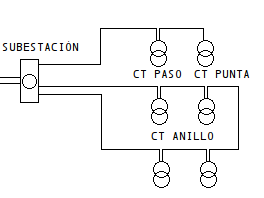
\includegraphics[width=0.5\linewidth]{cts}
\end{figure}

\subsubsection{Por la propiedad}

\begin{itemize}
	\item Un CT \textbf{de compañía} pertenece a la empresa distribuidora de energía, por lo que de él parten las redes públicas de distribución en \acrshort{bt}.
	\item Un CT \textbf{de cliente} es propiedad del cliente y debe realizar la medida de la energía eléctrica:
	\begin{itemize}
		\item En centros de transformación de pequeña potencia se realiza en el lado de \acrshort{bt}, para no medir la energía perdida en la transformación.
		\item En centros de transformación de mayor potencia se realiza en el lado de \acrshort{mt}, con parte de las celdas de \acrshort{mt} de la compañía distribuidora.
	\end{itemize}
\end{itemize}

\subsubsection{Por el emplazamiento}

\begin{itemize}
	\item Un CT \textbf{de intemperie} es aquel en el que todos sus elementos se ubican en el exterior. En ellos el transformador y el resto de elementos se suelen instalar sobre apoyos metálicos o de \acrshort{ha}.
	\item Un CT \textbf{de interior} es aquel en el que todos sus elementos están situados dentro de un local de distinta naturaleza, reservado para tal fin.
\end{itemize}

\subsubsection{Por el tipo de acometida}
\begin{itemize}
	\item Un CT \textbf{con cometida aérea} es aquel en el que la conexión a la red de distribución se realiza mediante cable aéreo desnudo. Es el sistema utilizado en los de intemperie y en algunos de interior.
	\item En un CT \textbf{con acometida subterránea} la conexión se realiza mediante cables aislados en zanja. La mayoría de los centros de transformación de interior son de este tipo.
\end{itemize}

\subsubsection{Por la obra civil}

\begin{itemize}
	\item Un CT \textbf{convencional} es aquel que se ubica en el interior de recintos diseñados según proyecto de obra civil.
	\item Un CT \textbf{prefabricado} es aquel que dispone de una envolvente de hormigón armado hecha con módulos o con bloques por un fabricante específico. Son habituales, ya que tienen tamaño reducido, son fáciles de transportar e instalar y presentan otros beneficios.
	\item Un CT \textbf{subterráneo} es aquel en el que todos los elementos se encuentran en un recinto subterráneo. Presentan algunas ventajas como la reducción del impacto visual y ambiental, la optimización del espacio, la mayor seguridad frente a actos vandálicos o accidentes y la menor exposición a las condiciones climáticas. Sin embargo, su diseño, instalación y mantenimiento requieren una mayor planificación y cuidado
\end{itemize}

\subsection{Celdas en los CT}

Una \textbf{celda} se puede definir como un bloque con una función independiente que forma parte del centro de transformación. Las celdas se componen de elementos de conmutación, control, medida y/o protección.

Las celdas más habituales, según la función que desempeñan, son:
\begin{itemize}
	\item Las celdas \textbf{de línea} (normalmente 1, 2 o 3), tienen la función de permitir la entrada y salida en el CT de las líneas de \acrshort{mt}.
	\item Las celdas \textbf{de protección}, permiten ubicar la aparamenta de protección general y de cada transformador.
	\item Las celdas \textbf{de medida}, utilizadas en los CT de abonado, albergan los transformadores de intensidad y tensión.
	\item Las celdas \textbf{de remonte}, permiten la separación física entre la parte del CT manipulada sólo por la compañía y la parte manipulada por el cliente, en los CT de abonado.
	\item Las celdas \textbf{de seccionamiento}, en ella se encuentran los elementos de apertura de las diferentes líneas de tensión.
\end{itemize}

La ETN 44 \cite{etn-44} especifica los tipos de celdas para distribución secundaria, tipo interior para 13,2 y 33 kV, y detalla los equipos que componen a cada una.

\subsection{Esquemas unifilares}

\subsubsection{CT de compañía}

Utiliza celdas de línea y celdas de protección.

Los esquemas básicos para estos CT de compañía son:
\begin{itemize}
	\item En punta: tienen celda de línea y de protección según la cantidad de transformadores (figura \ref{fig:ct-compañia-a}).
	\item En bucle: tienen celdas de entrada y salida, y de protección según la cantidad de transformadores (figura \ref{fig:ct-compañia-b}).
\end{itemize}

% Figura ct-compañia

\subsubsection{CT de abonado}

Como el CT de compañía, utiliza celdas de línea y protección, pero además como mínimo debe incluir también una celda de medida. 

Los esquemas típicos son:
\begin{itemize}
	\item En punta: cuentan con una celda de línea, de medida y de protección (figura \ref{fig:ct-abonado-a}).
	\item En bucle: con celdas de línea da continuidad a la línea de distribución en \acrshort{mt} y, además, se separaran eléctricamente mediante celdas de remonte. Tienen celdas de protección según la cantidad de transformadores (figura \ref{fig:ct-abonado-b}).
\end{itemize}

% Figura ct-abonado

La ETN 99 (\cite{etn-99}) especifica la construcción de las celdas correspondientes a la compañía en los CT de abonado, dependiendo de la zona, el cliente y la demanda convenida (tabla \ref{tab:tipo-ct-epe}).

% tabla tipo-ct-epe
\begin{longtable}{cc|c|c|c|c|c}
	\caption{Instalaciones según el tipo de cliente y las demandas convenidas.}\label{tab:tipo-ct-epe} \\ \hline
	\multirow{2}{*}{Cliente} & \multirow{2}{*}{Zona de Ubicación} & \multicolumn{5}{c}{Tipo de instalación según demanda convenida.} \\  
	& &  & $\geq$ 300 kW & $\geq$ 500 kW & $\geq$ 1000 kW & $\geq$ 2000 kW \\ \hline
	\endfirsthead
	
	\multicolumn{7}{l}{\cabezaTabla{tab:tipo-ct-epe}} \\ \hline
	\multirow{2}{*}{Cliente} & \multirow{2}{*}{Zona de Ubicación} & \multicolumn{5}{c}{Tipo de instalación según demanda convenida.} \\  
	& &  & $\geq$ 300 kW & $\geq$ 500 kW & $\geq$ 1000 kW & $\geq$ 2000 kW \\ \hline
	\endhead
	
	\hline \multicolumn{7}{r}{\pieTabla} \\  
	\endfoot
	
	\hline
	\endlastfoot
	
	\multirow{2}{*}{GC} & Rural     &  & PAMMF & \multicolumn{3}{c}{CMMI} \\  \cline{4-7} 
	& No rural  &  & \multicolumn{2}{c|}{CMMF} & \multicolumn{2}{c}{CMMI} \\ \hline
	\multirow{2}{*}{CCoop} & Rural  & \multicolumn{2}{c|}{PAMMF} & \multicolumn{2}{c|}{PAMMR} & CMMI \\ \cline{3-7}  
	& No rural & PAMMF & \multicolumn{3}{c|}{PAMMR} & CMMI \\  
\end{longtable}


Donde se tienen las siguientes siglas:
\begin{itemize}
	\item Grandes Clientes (GC) y Clientes Cooperativas (CCoop). 
	\item Cabina de Maniobras y Medición (CMM), con fusibles (F) o Interruptor (I).
	\item Puesto Aéreo de Maniobra y Medición (PAMM), con fusibles (F) o Reconectador (R).
\end{itemize}

% Ejemplo de lo que hicimos en nuestro trabajo práctico
La Figura \ref{fig:ejemplo-ct} muestra el CT que realizamos con mi grupo para una industria donde se proyectó la instalación de dos transformadores de 800 kVA cada uno.

\begin{figure}[!h]
	\centering
	\caption{Ejemplo de CT de abonado. Cada celda indica su función.}
	\label{fig:ejemplo-ct}
	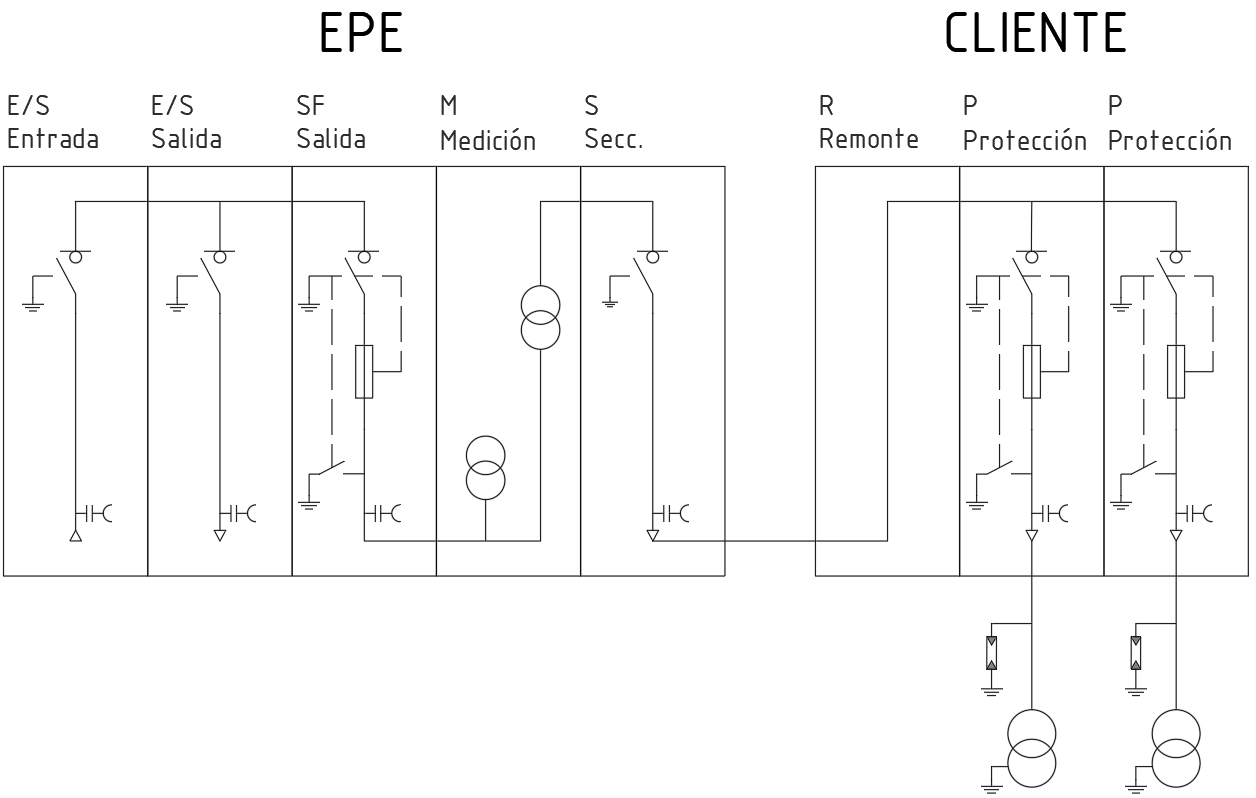
\includegraphics[width=0.9\linewidth]{ct-abonado}
\end{figure}